\section{Quarkonium production}
\label{sec:qurkonia}
Measurements of quarkonium production promise to yield important information about the
strongly-interacting system formed in heavy-ion collisions.  
The in-medium dissociation of quarkonium states in these collisiosn due to color-screening effects
is expected to reflect both the state's binding energy as
well as the temperature and other properties of the medium, leading to a characteristic
suppression or disappearance pattern of the various charmonium and 
bottomonium states~\cite{Matsui:1986dk,Digal:2001ue,Mocsy:2007jz}.

\jpsi\ production in heavy-ion collisions has been studied over a wide range of
collision energies at the CERN SPS and RHIC, with a strong suppression of \jpsi\
yields observed in central collisions for $\rootsNN \approx 20$ to
$200$~GeV~\cite{Baglin:1994ui,Alessandro:2004ap,Alessandro:2006ju,Adare:2006ns,
Arnaldi:2007zz,Adare:2011yf}.
The interpretation of the observed suppression is complicated by the presence
of Cold Nuclear Matter (CNM) effects such as nuclear absorption and nuclear
modifications of parton distribution functions. A quantitative
description furthermore needs to take into account feeddown from excited states,
which contribute a significant fraction of the inclusive \jpsi\ yield in \pp\ collisions.
Finally, and perhaps most importantly, the large abundance of deconfined charm quarks
at RHIC and higher energies requires the consideration of a recombination 
component of the observed \jpsi\ yield, in addition to direct \jpsi\ production, which 
may mask the suppression of the initial
\jpsi\ formation~\cite{BraunMunzinger:2000px,Thews:2000rj,Zhao:2007hh,Capella:2007jv}.

The large increase in the charm cross-section at LHC should magnify these recombination
effects compared to lower energy collisions. This provides the opportunity to separate
dissociation and recombination effects by studying \jpsi\ suppression
as a function of collision energy, \pT\ and rapidity, where these parameters
control both the properties of the local medium and the density of charm quarks.

The LHC collision energies also facilitate high statistics studies of the \PgU\ family, where
the three \PgUn\ states are connected by the common initial bottom pair production,
but distinguished by the hierarchy of their binding energies. In an
in-medium dissociation picture, one therefore expects a distinct pattern in the suppression
of the \PgUn\ states reflecting their different binding energies.

\subsection{Charmonium suppression}

J/$\psi$ production in \PbPb\ collisions can be characterized relative to \Ncoll-scaled \pp\ or 
peripheral \PbPb\ reference
distributions, using the \Raa\ and \Rcp\ nuclear modification factors introduced earlier.
A strong suppression of high-\pT\ inclusive \jpsi\ in the dimuon decay channel 
was observed in 2.76\TeV\ \PbPb\ collisions by all three LHC experiments over a wide 
range in transverse momentum, using a peripheral \PbPb\ reference in ATLAS~\cite{Aad:2010aa} 
and a \pp\ reference in CMS~\cite{Chatrchyan:2012np} and ALICE~\cite{Abelev:2012rv}.

Results for the suppression of low \pT\ \jpsi\ production from ALICE are shown
in Fig.~\ref{fig:GR:raavsy} for $\pT > 0$\GeVc\ (square markers) and
$\pT > 3$\GeVc\ (diamond markers), together with CMS data~\cite{Chatrchyan:2012np} (triangle markers)
for rapidity $ 1.6 < |y| < 2.4 $ and $\pT > 3$\GeVc.

\begin{figure}
\begin{center}
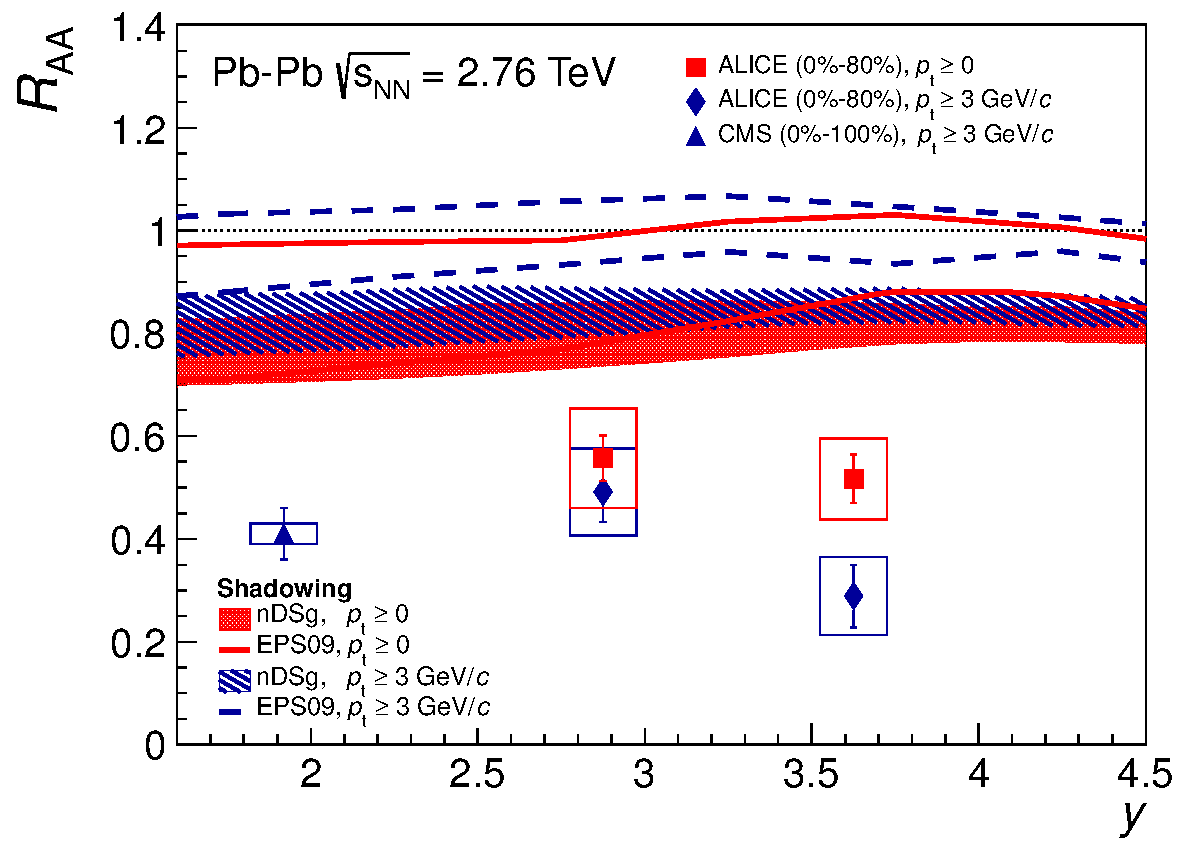
\includegraphics[width=0.49\linewidth]{qqbarfigures/RAAvsY_v7-eps-converted-to.pdf}
\caption{ \label{fig:GR:raavsy}  Inclusive \jpsi\ \Raa\ measured in 2.76~TeV \PbPb\
collisions as a function of  rapidity for two \pT\ ranges.
Systematic uncertainties are displayed as open boxes. 
Uncertainties on the \pp\ luminosity and \Taa\ scaling factor of
5.2\% and  8.3\% for ALICE and CMS, respectively, are not included.
Two model predictions are shown~\cite{Ferreiro:2011rw,Vogt:2010aa}, including only shadowing effects
for  nDSg (shaded areas) and EPS09 (lines) nPDFs. Reproduced from~\cite{Abelev:2012rv}.}
\end{center}
\end{figure}

Within uncertainties, neither \pT\ range shows a strong dependence of \jpsi\ suppression on rapidity.
The suppression is stronger than predicted for shadowing effects in the Color Singlet
Model~\cite{Ferreiro:2011rw} and the Color Evaporation Model~\cite{Vogt:2010aa}. 

While neither model, nor the data, show a strong rapidity dependence, more decisive 
information can be expected from the \pT\ dependence of \Raa\. Here initial state 
suppression models typically expect the strongest suppression effects at low \pT, while 
regeneration models expect the largest enhancement from charm recombination in that \pT\ range,
reflecting the charm quark phase-space density.
These expectations can be confronted with data from ALICE and CMS on the \pT\ dependence of the 
\jpsi\ \Raa\ over a wide range \pT\ range shown in Fig.~\ref{fig:GR:raaexp2}. 
Although the ALICE and CMS measurements cover different rapidity ranges ($2.0 < |\y| < 4.0$ vs.\ $ 1.6  < |\y| < 2.4 $)
a common, strong \pT\ evolution of \jpsi\ \Raa\ is seen, ranging from $\approx 0.8$ 
at low \pT\ to $\approx 0.4$ for $\pT > 5$\GeVc.
This observation clearly favors models including a low-\pT\ enhancement due to charm recombination.

An even more striking observation is shown in the right panel of Fig.~\ref{fig:GR:raaexp2}, which compares
the ALICE forward-rapidity \jpsi\ \Raa\ for central 2.76\TeV\ \PbPb\ collisions~\cite{Abelev:2013ila}
with central 200\GeV\ \AuAu\ data from PHENIX measured in $1.2 < |\y| < 2.2$~\cite{Adare:2011yf}.
At low \pT\ the ALICE \Raa\ is about four times larger than that seen at the lower energy (i.e.,
there is much less suppression seen at LHC than at RHIC), while
at the same time the initial energy density of the system at LHC is estimated to be larger than at
RHIC by a similar factor. While a quantative interpretation of this result will require
a detailed understanding of CNM effects at the two energies, the results are  consistent
with the collision energy trend expected in recombination approaches such as~\cite{Zhao:2007hh,Zhou:2013aea,Liu:2009nb}.
First results on \jpsi\ production in \pPb\ collisions at the LHC have recently
been presented~\cite{Abelev:2013yxa,Aaij:2013zxa}, allowing
the calibration of CNM effects vs.\ final state suppression and recombination.

\begin{figure}[h!]
\begin{center}
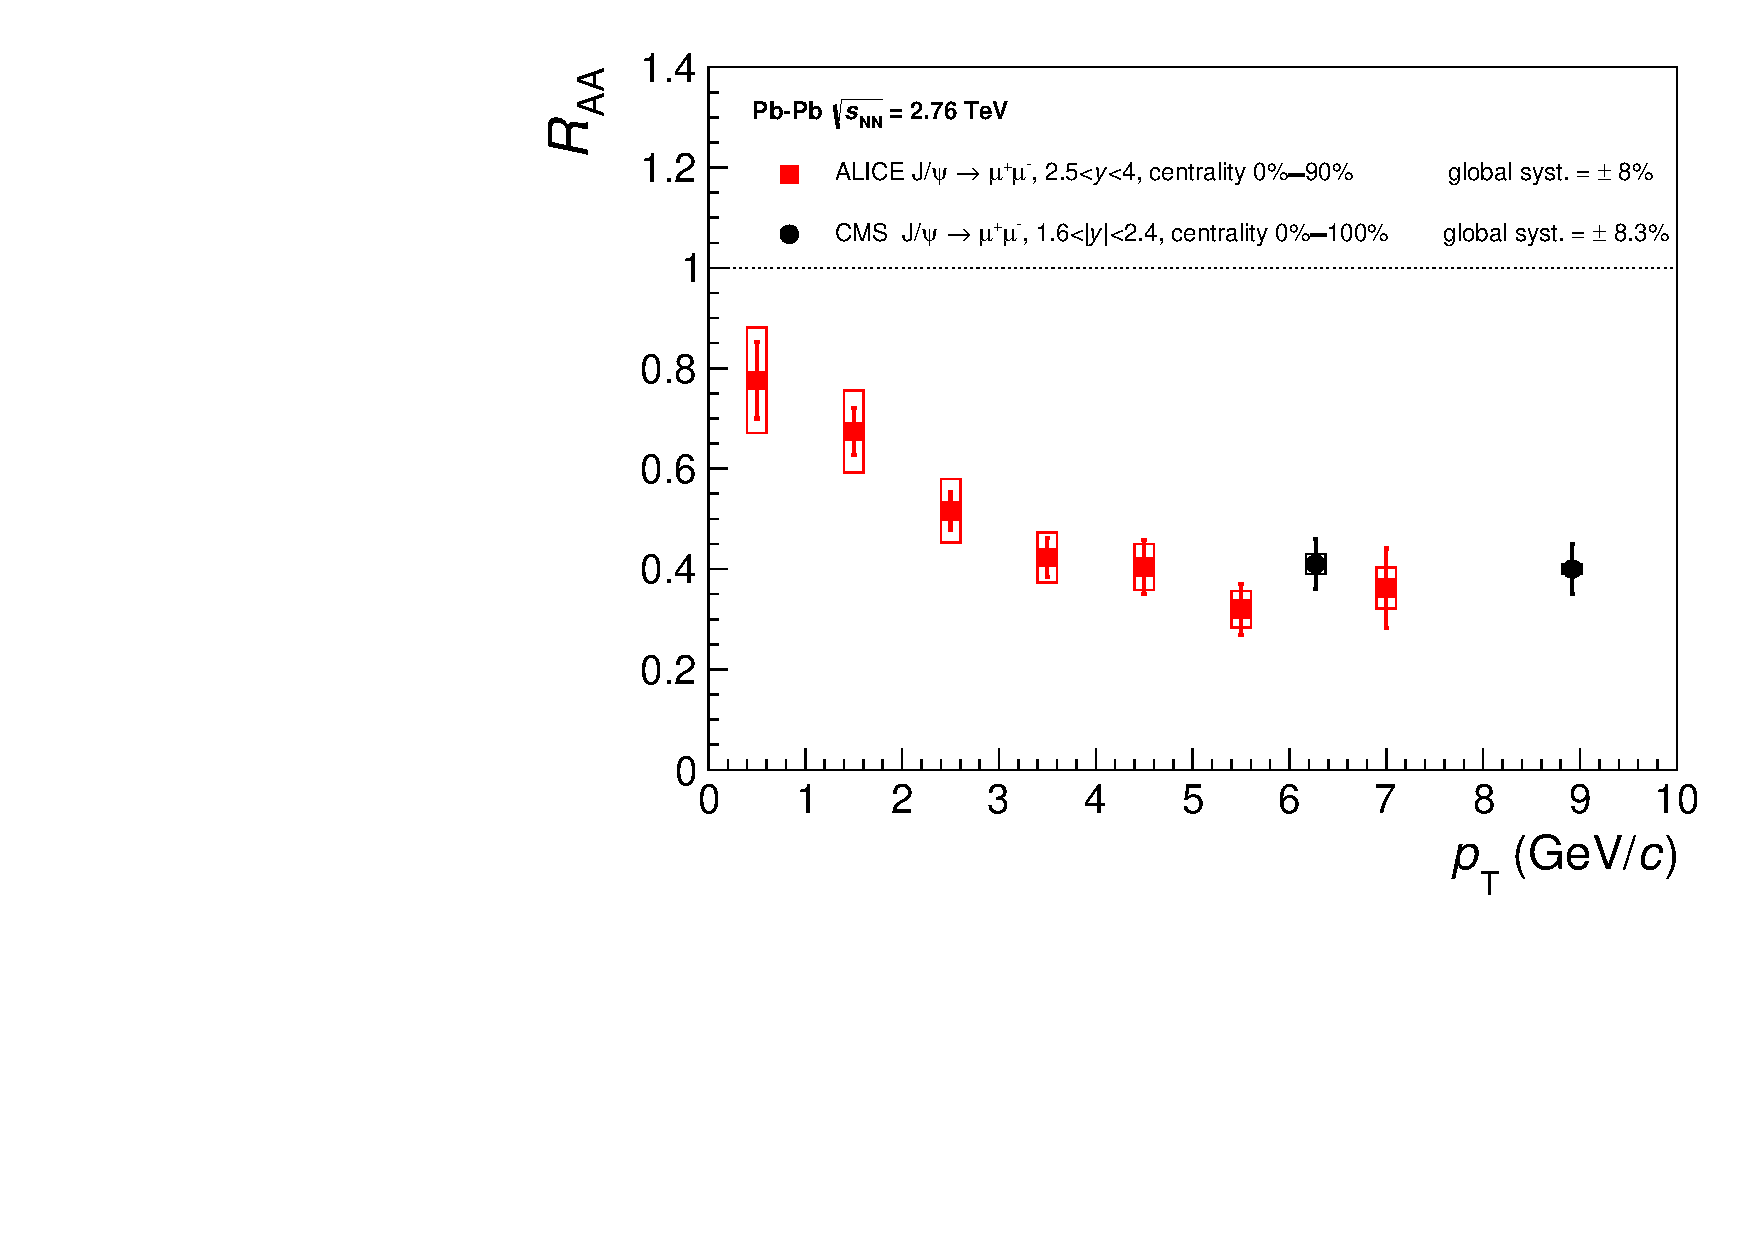
\includegraphics[width=0.49\linewidth,keepaspectratio]{qqbarfigures/RAAPtvsModels1.pdf}
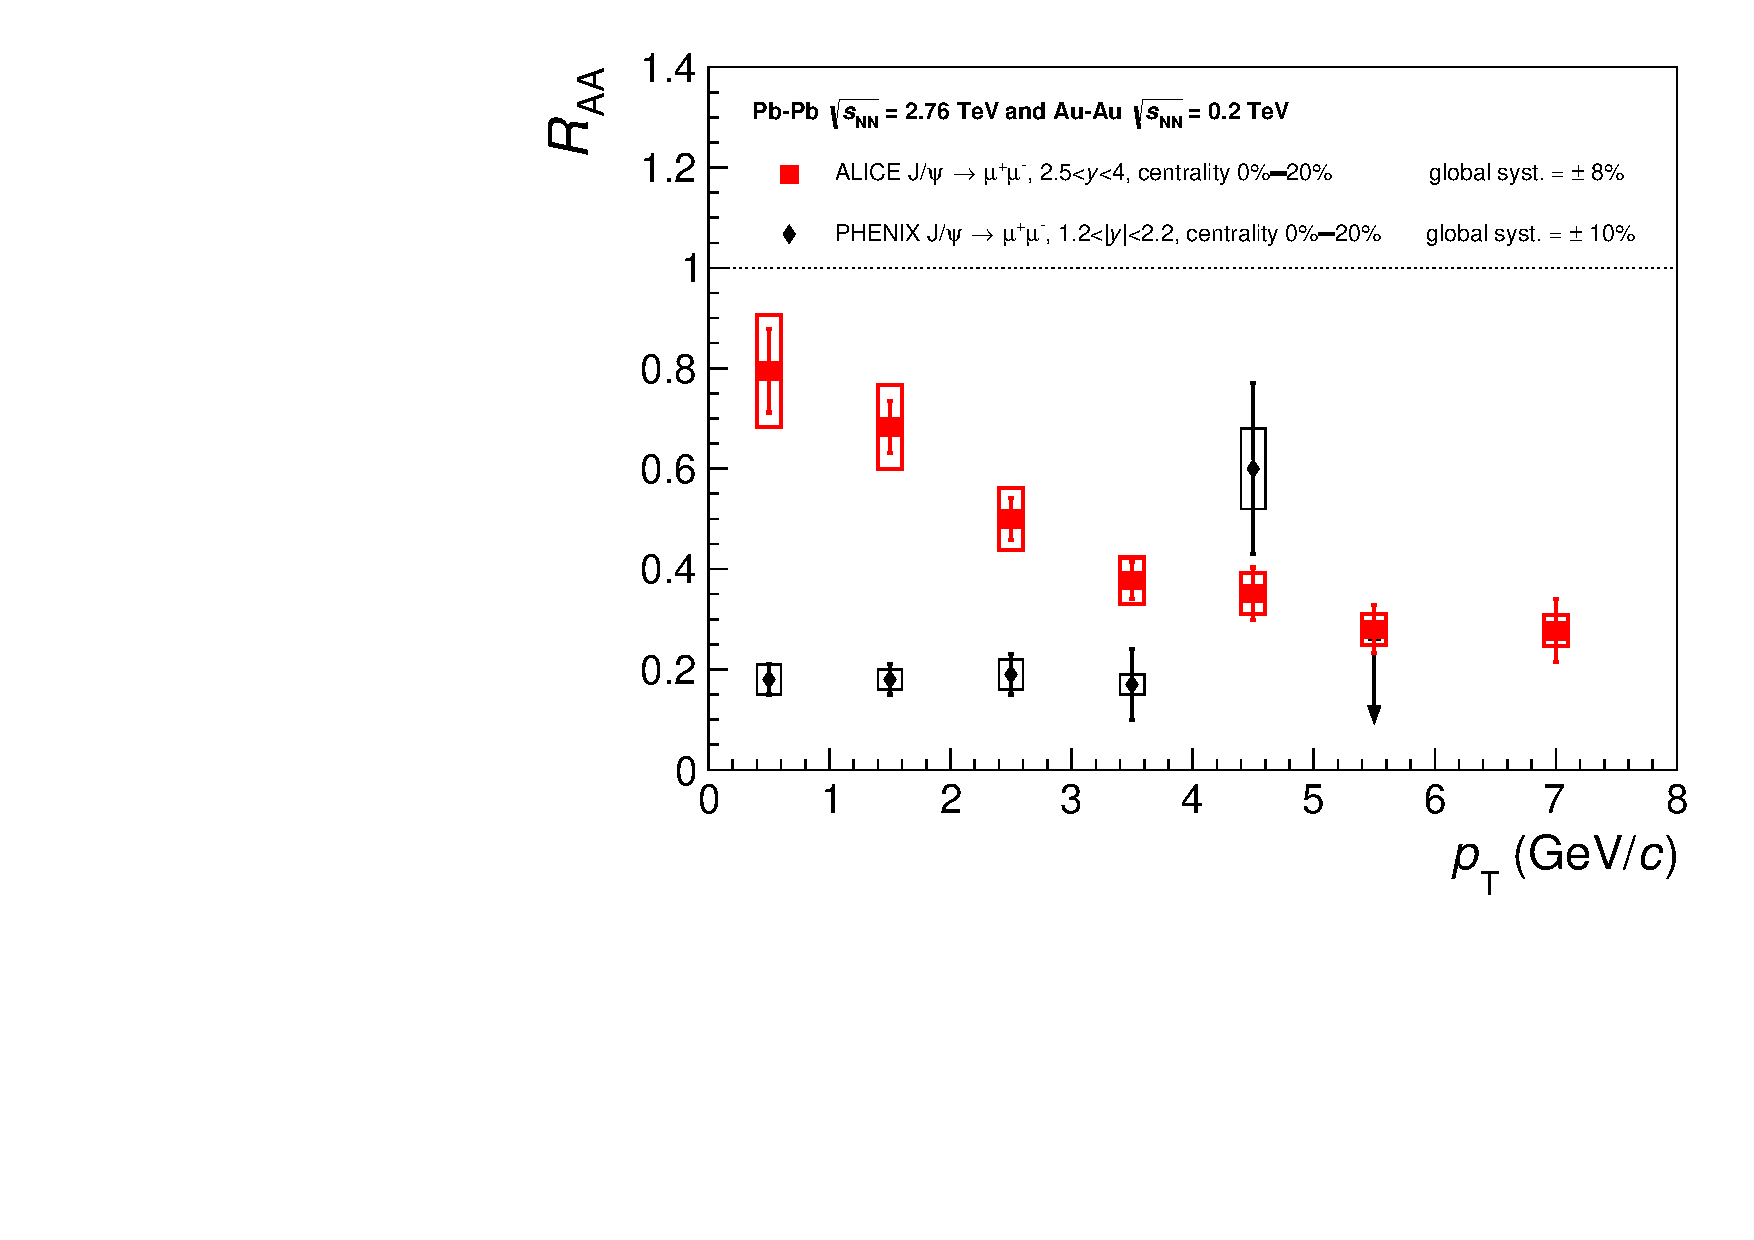
\includegraphics[width=0.49\linewidth,keepaspectratio]{qqbarfigures/RAAPtvsModels2.pdf}
\caption{ \label{fig:GR:raaexp2}
(left) \pT\ dependence of \jpsi\ \Raa\ measured by ALICE in 2.76~TeV \PbPb\
collisions (0--80\% centrality) compared to CMS~\cite{Chatrchyan:2012np}
results (0--100\% centrality).
(right) \pT\ dependence of \jpsi\ \Raa\ measured by ALICE 
in 2.76\TeV\ \PbPb\ collisions compared to PHENIX~\cite{Adare:2011yf}
results in 200\GeV\ \AuAu\ collisions, both for 0--20\% centrality.  Reproduced from~\cite{Abelev:2013ila}}
\end{center}
\end{figure}


\subsection{Charmonium elliptic flow}

An important question for models implementing the competing contributions of
\jpsi\ dissociation in the medium and \jpsi\ regeneration via charm quark recombination is
the degree of charm quark thermalization. The question of thermalization in heavy-ion 
collisions is typically addressed via studies of hydrodynamic flow. 
ALICE has recently presented the first data 
suggesting non-zero elliptic flow in \PbPb\ collisions~\cite{ALICE:2013xna} at LHC, 
providing important information on this topic.

In a dissociation/recombination type approach, elliptic flow of the observed \jpsi\ can 
arise from multiple contributions. Initially produced \jpsi\ traverse a shorter path 
in the medium (and hence are less likely to be dissociated) when travelling in-plane vs 
out-of-plane, leading to a possible azimuthal modulation of \jpsi\ yields with respect 
to the event plane. If charm quarks participate in the collective expansion of the medium, as
suggested by the observed elliptic flow of open charm mesons, \jpsi's produced by recombination will
pick up the elliptic flow of these charm quarks. The various contributions can possibly be disentangled 
by studies of the \pT\ dependence of \jpsi\ suppression and \jpsi\ elliptic flow.

\begin{figure}
\begin{center}
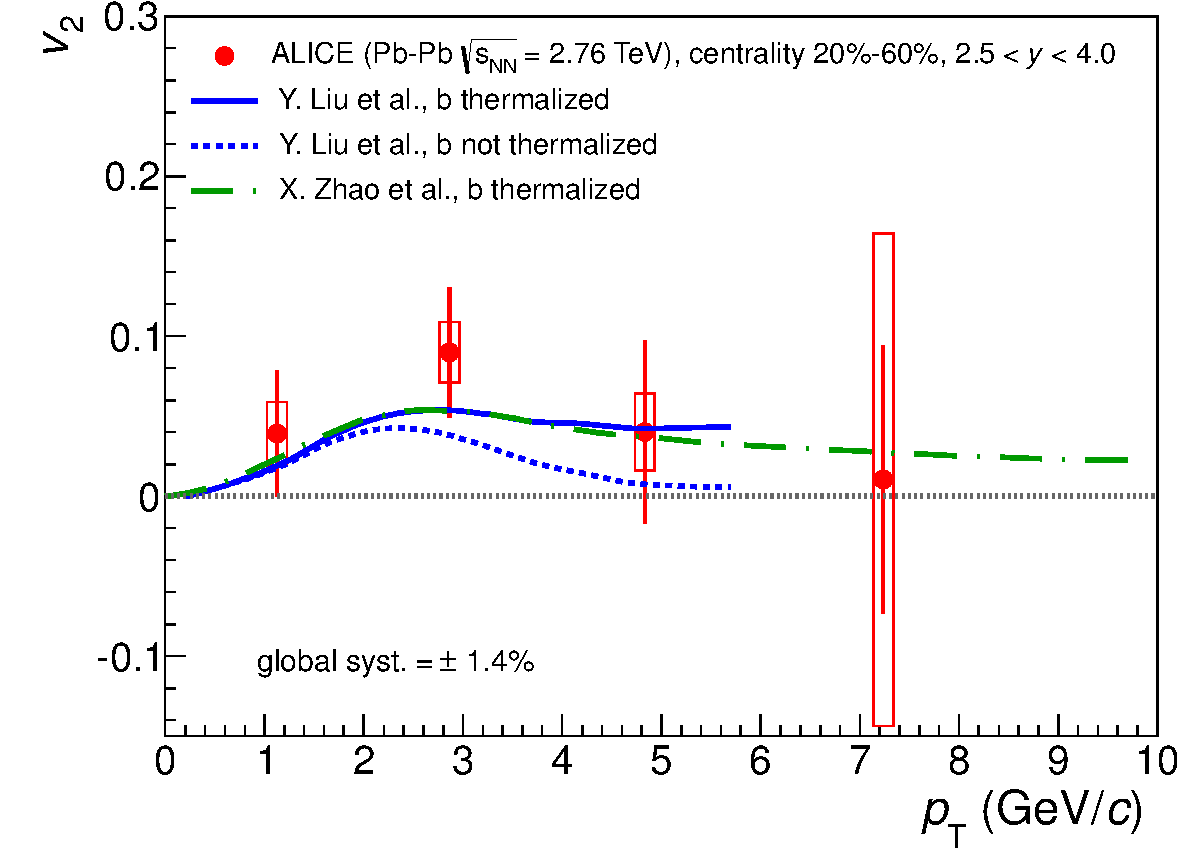
\includegraphics[width=0.49\linewidth]{qqbarfigures/prl_fig4-eps-converted-to.pdf}
\caption{\label{fig:GR:v2ptcomp} Inclusive \jpsi\ \vtwo\
for 2.76\TeV\ \PbPb\ collisions with 20--60\% centrality as a function of \pT.
Data are compared to calculations from two transport models~\cite{Liu:2009gx,Zhao:2012gc}. 
Reproduced from~\cite{ALICE:2013xna}}
\end{center}
\end{figure}
Previous measurements of the \jpsi\ elliptic flow by STAR for \AuAu\ collisions at 
$\rootsNN = 200$\GeV are consistent with zero~\cite{Adamczyk:2012pw}, 
altough the large uncertainties prevent strong conclusions.
In contrast, the ALICE measurement yielding a non-zero value of \jpsi\ \vtwo\ as a function 
of transverse momentum is shown in Fig.~\ref{fig:GR:v2ptcomp} for \PbPb\ collisions in the 20--60\% 
centrality range~\cite{ALICE:2013xna}.
The \jpsi\ \vtwo\ data, for which ALICE quotes a significance of about 2$\sigma$ in this centrality range, 
are compared to transport model calculations~\cite{Liu:2009gx,Zhao:2012gc}. 
The models, which include charm quark recombination effects,
are both compatible with the data within the current large experimental uncertainties. 
The comparison points to the importance of future high statistics measurements 
of \jpsi\ elliptic flow at high transverse momentum ($\pT > 5$\GeVc).

In combination, the \pT\ and collision energy dependence of \jpsi \Raa\ and 
the indication of non-zero \jpsi\ elliptic flow suggest a possible  
contribution of charm quark recombination to \jpsi\ production in \PbPb\ collisions
at LHC.

\subsection{Upsilon suppression}

Measurements by CMS have provided the first high statistics look at \PgU\
production in heavy-ion collisions~\cite{CMS_Y_2010}.
The \PgU\ family presents an ideal system to test in-medium dissociation effects,
as the three states have similar decay kinematics, but a large variation of binding energies,
Compared to charmonium suppression studies, uncertainties due
to CNM effects and recombination effects are expected to be
less important for the bottomonium family.

Dimuon invariant mass spectra in the \PgU\ mass range obtained by CMS are shown in 
Fig.~\ref{fig:GR:mass} for \PbPb\ (left) and \pp\ (right)~\cite{Chatrchyan:2012lxa}
at 2.76~TeV collision energy for both systems. 
The data correspond to integrated luminosities of $150\mubinv$ and $230 \nbinv$ for
\PbPb\ and \pp, respectively. For the \pp\ data, the excellent mass resolution of the CMS muon system
allows a clear separation of the three \PgUn\ states. A similar mass resolution is achieved 
for \PbPb\ collisions.
However, for \PbPb\ a strong suppression of the \PgUb\ state is evident from the 
distribution, and the \PgUc\ state is no longer visible above the continuum background. 
This is a striking visual confirmation of the expected
\PgU\ suppression pattern as a function of the \PgUn\ binding energy, and confirmed the 
first \PgU\ measurements reported in~\cite{CMS_Y_2010}.

\begin{figure}[t]
\begin{center}
    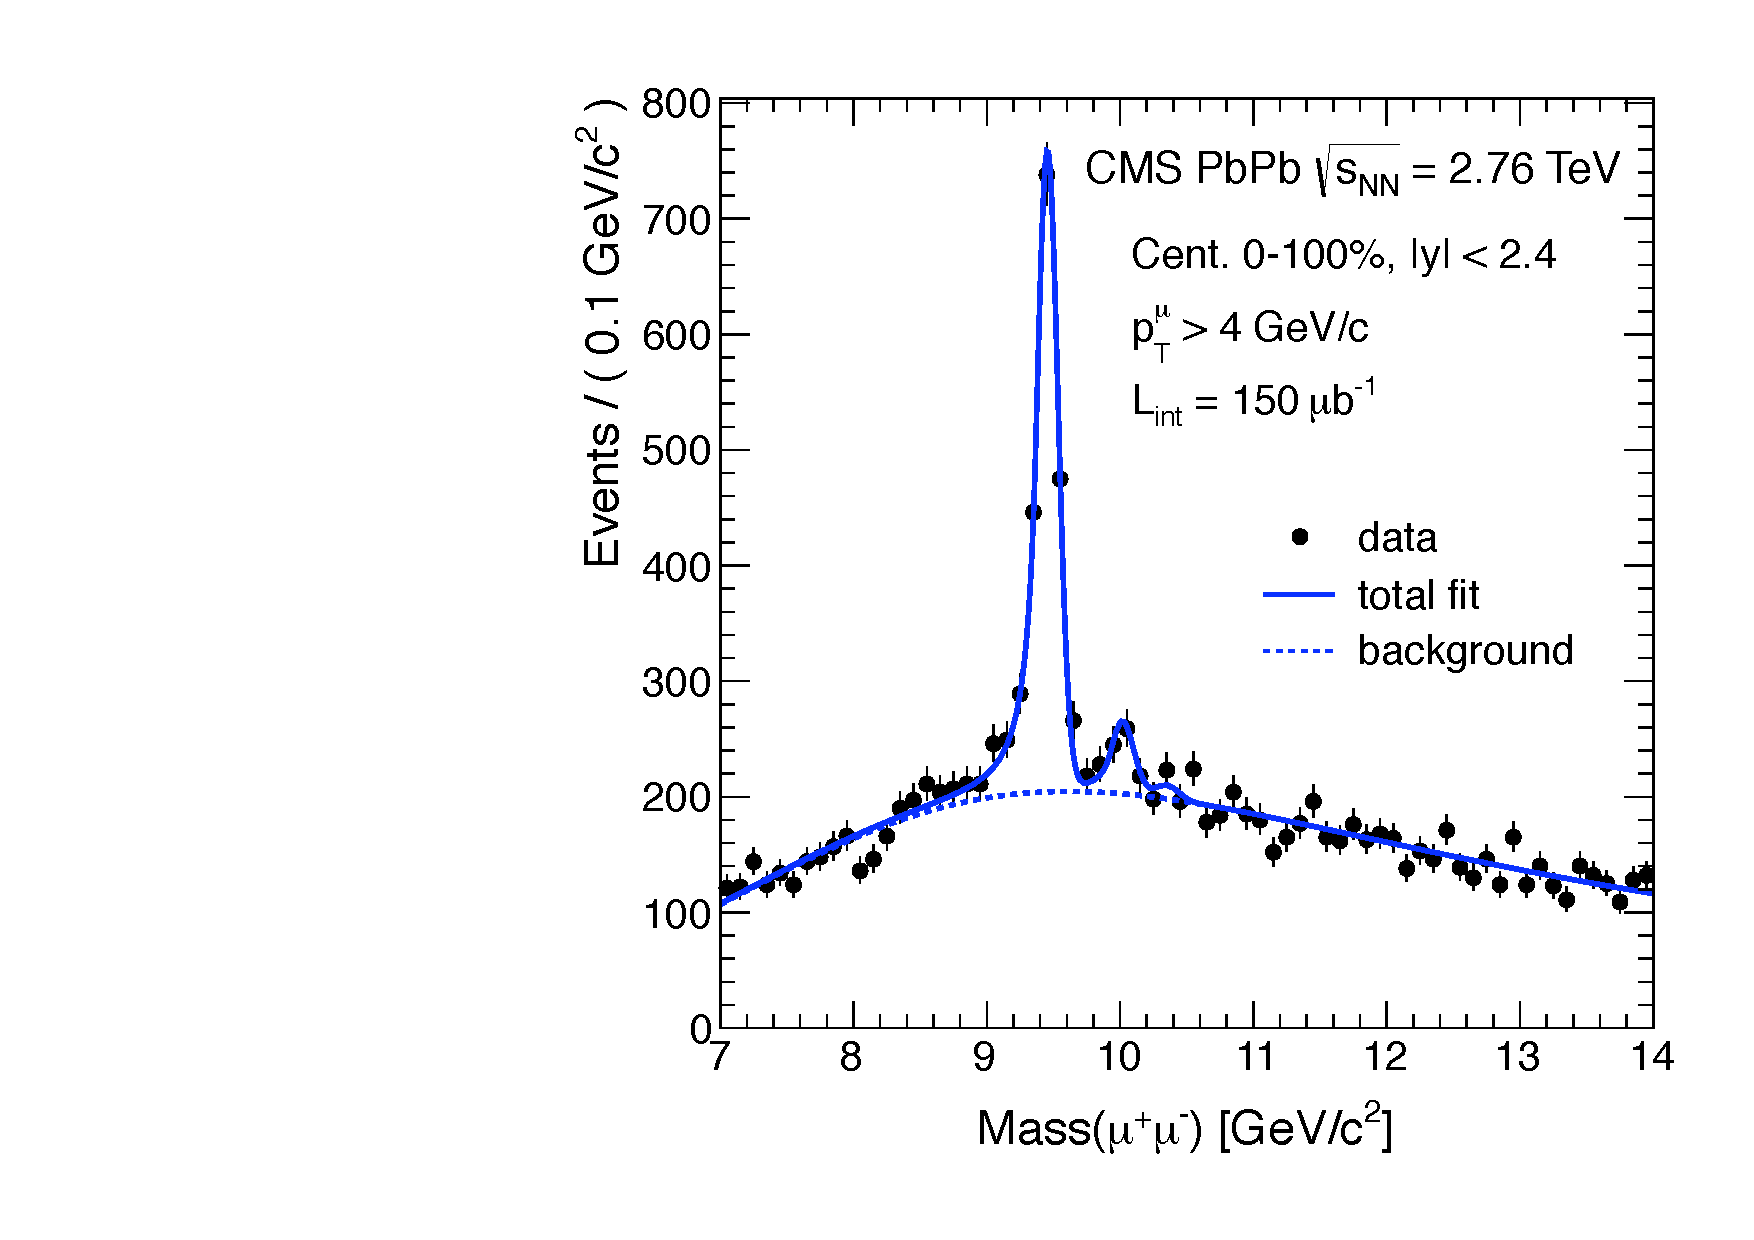
\includegraphics[width=0.45\textwidth]{qqbarfigures/hiFitPt4Erf}
    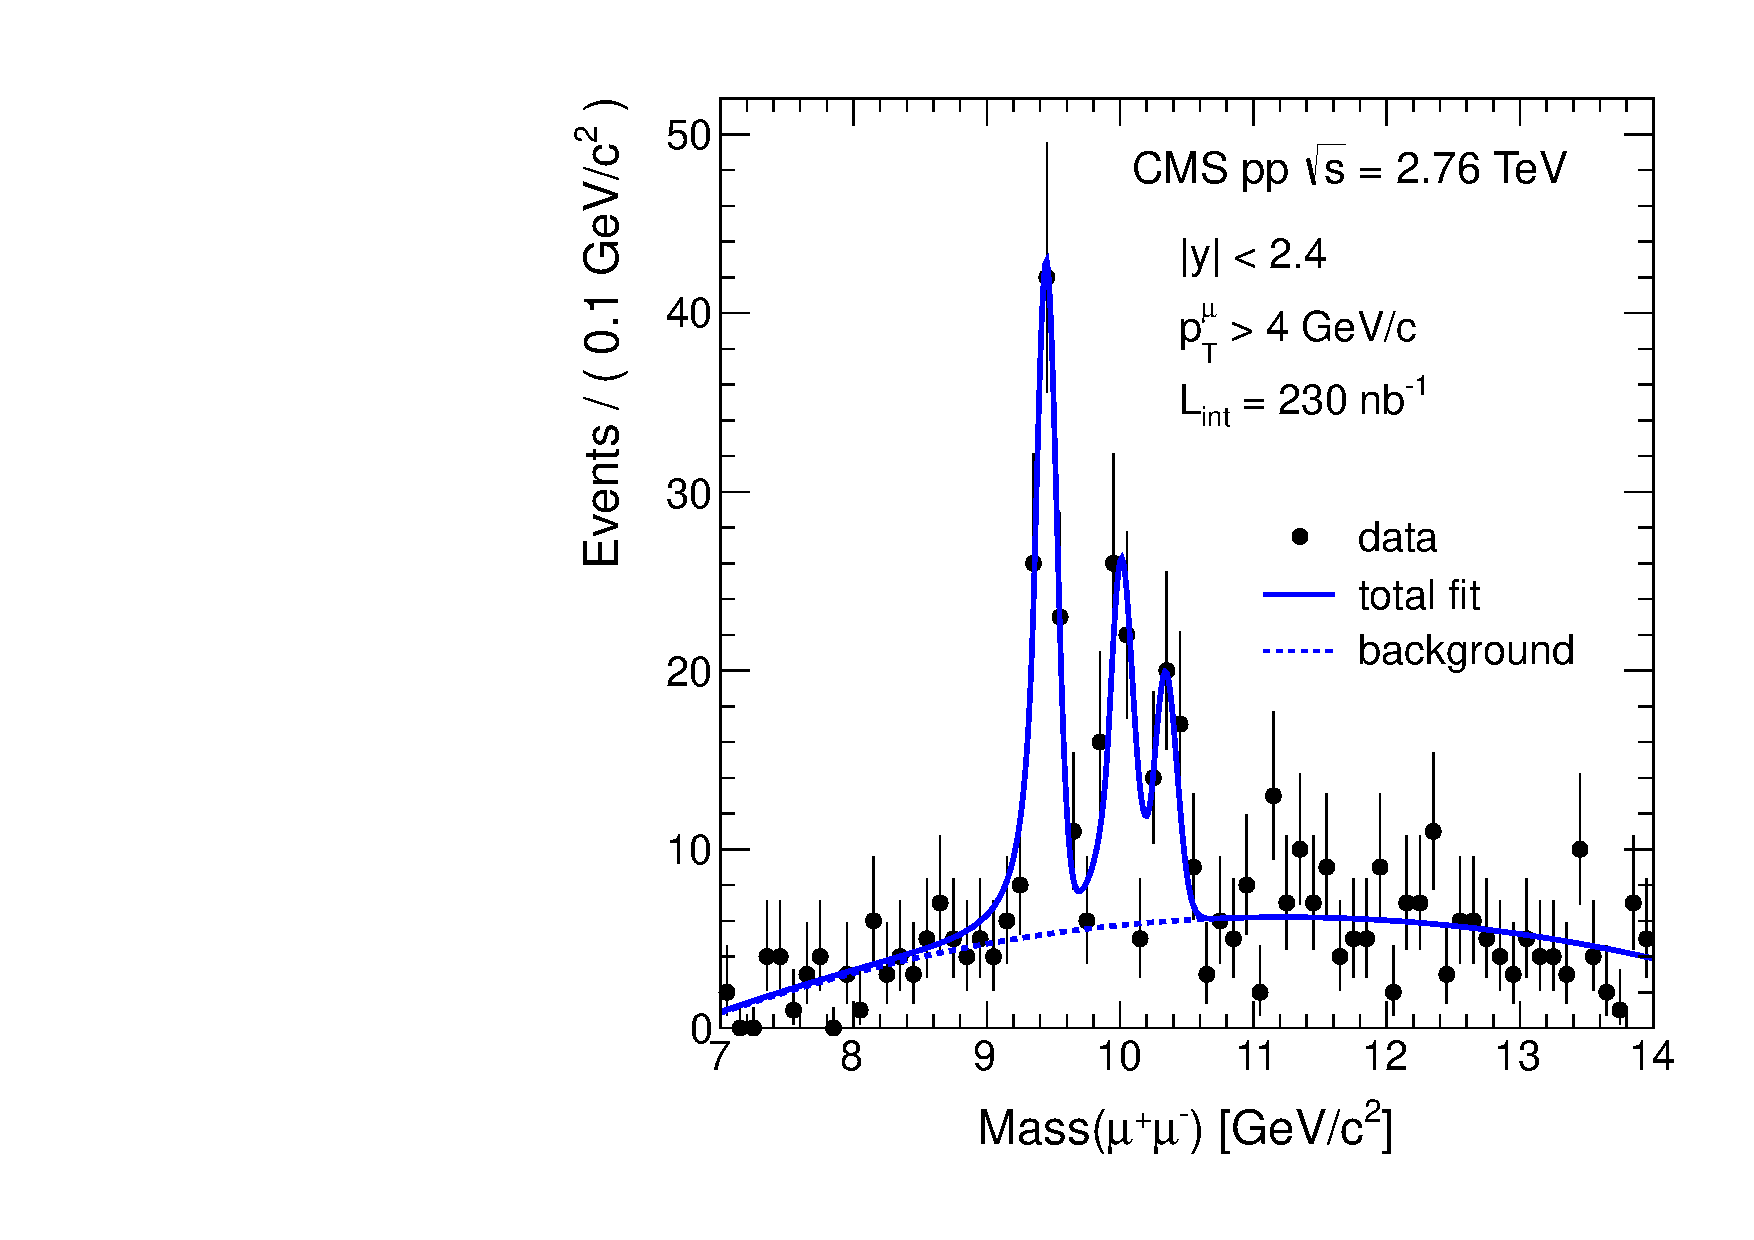
\includegraphics[width=0.45\textwidth]{qqbarfigures/ppFitPt4Erf}
    \caption{Dimuon invariant-mass distributions in 2.76\TeV\ \PbPb\ (left) and \pp\ (right)
collisions.  Lines show simultaneous fits to both
datasets for signal + background (solid) and background-only (dashed).
Reproduced from~\cite{Chatrchyan:2012lxa}}
\label{fig:GR:mass}
\end{center}
\end{figure}

The comparison of \pp\ and \PbPb\ data allows a characterization of the \PgU\ suppression
in terms of the nuclear modification factor \Raa~\cite{Chatrchyan:2012lxa}.
Integrating over centrality, the following \Raa\ values were measured for the \PgUn states:
\begin{eqnarray}
\Raa (\PgUa) &=& 0.56 \pm 0.08\,\text{(stat.)} \pm 0.07\,\text{(syst.)} \,, \\
\Raa (\PgUb) &=& 0.12 \pm 0.04\,\text{(stat.)} \pm 0.02\,\text{(syst.)} \,, \nonumber \\
\Raa (\PgUc) &=& 0.03 \pm 0.04\,\text{(stat.)} \pm 0.01\,\text{(syst.)} .  \nonumber
\end{eqnarray}
The statistical significance of the \PgUc\ peak above the continuum is less than one standard deviation.
It should also be noted that there are significant feed-down contributions to
the \PgUa\ state that may reach $\approx 50\%$~\cite{Affolder:1999wm, Aaij:2012se}.
This could mean that directly produced \PgUa\ state are largely unsuppressed, with
the observed \PgUa\ \Raa\ of 0.56 reflecting the dissociation of the higher 
mass excited states~\cite{Chatrchyan:2012lxa}.

The \PgUa\ and \PgUb\ suppression was also studied as a function of centrality,
as shown in Fig.~\ref{fig:GR:centrality}.
Here the relative suppression of \PgUa\ and \PgUb\ is characterized by
the double ratio \linebreak $({\PgUb/\PgUa})_{\rm PbPb}/({\PgUb/\PgUa})_{\rm pp}$
(Fig.~\ref{fig:GR:centrality}, left) and the absolute suppression
of the two states is shown as \Raa\ vs centrality (Fig.~\ref{fig:GR:centrality}, right)).

\begin{figure}[t]
\begin{center}
   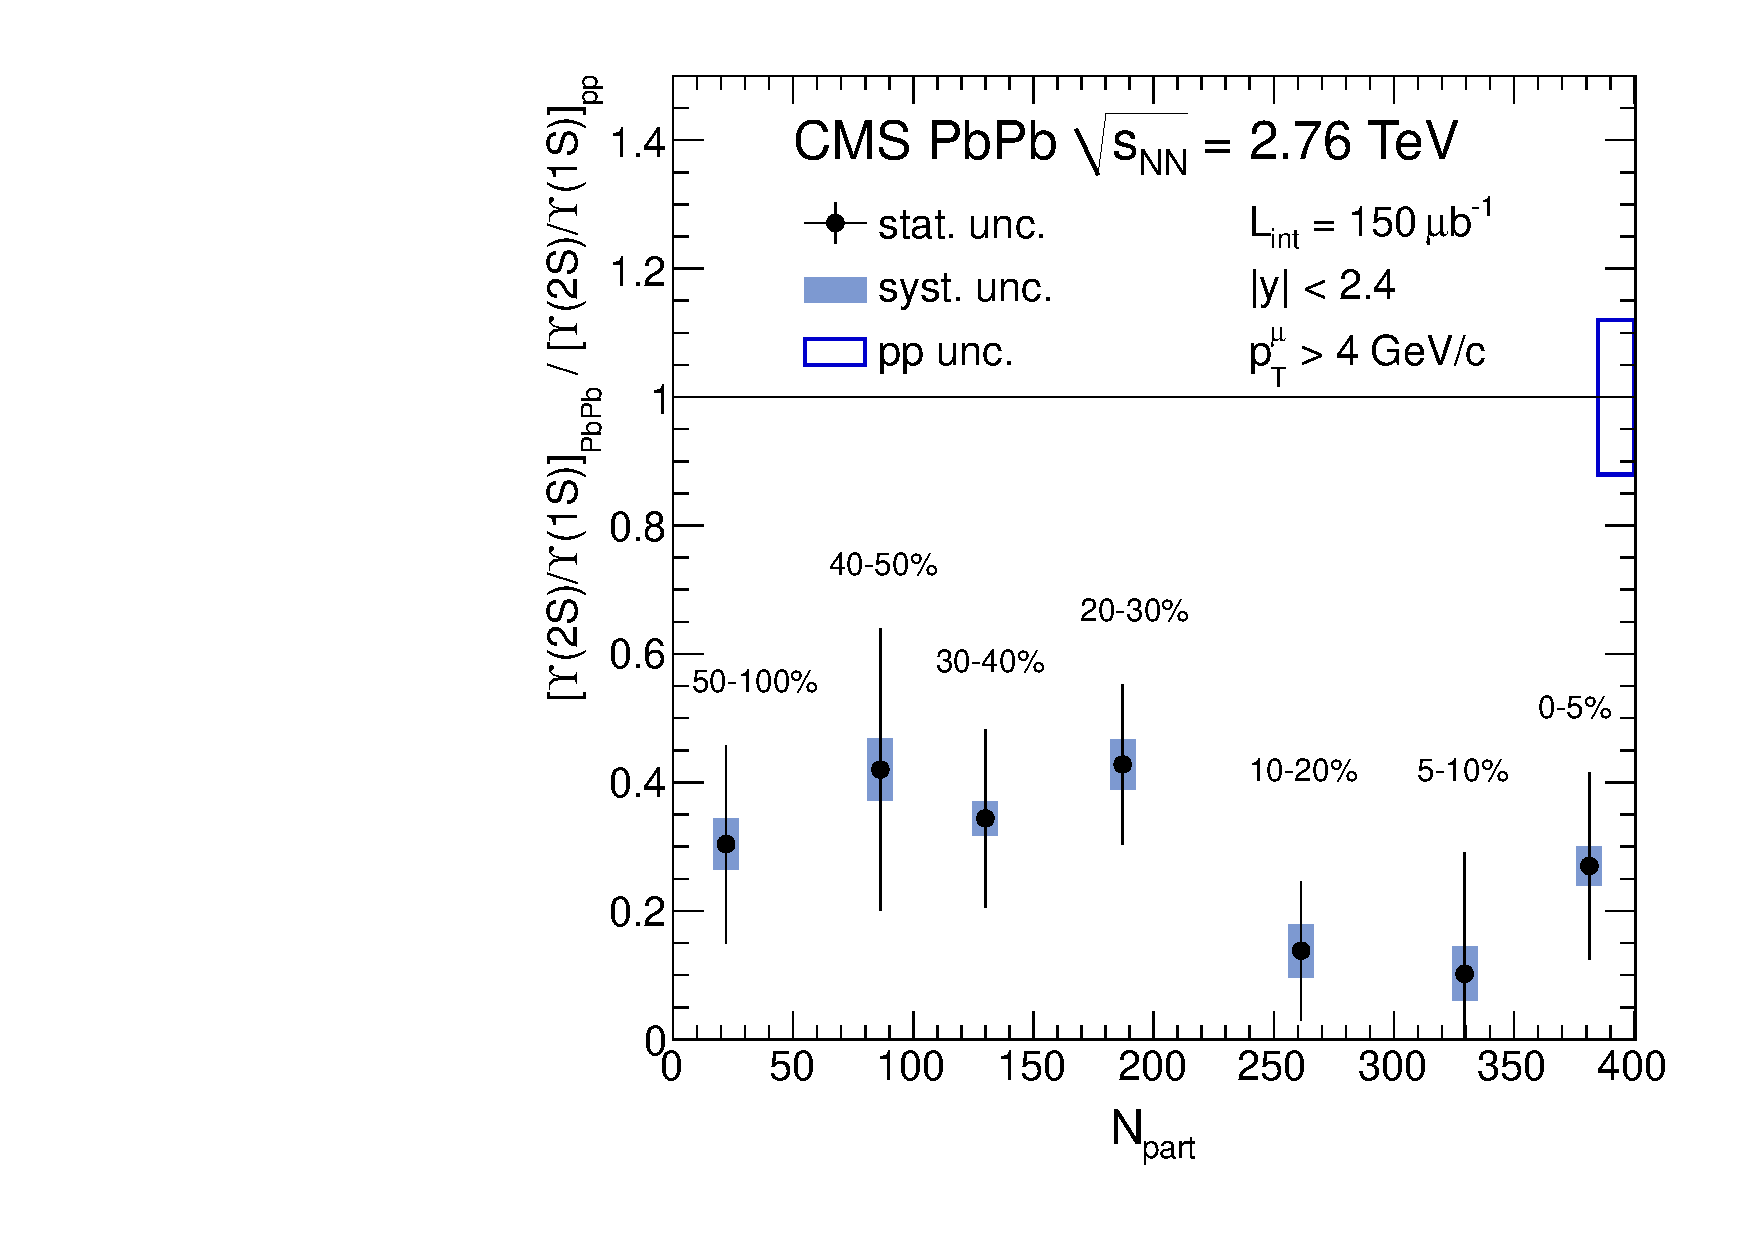
\includegraphics[width=0.45\textwidth]{qqbarfigures/chi2VsCent}
   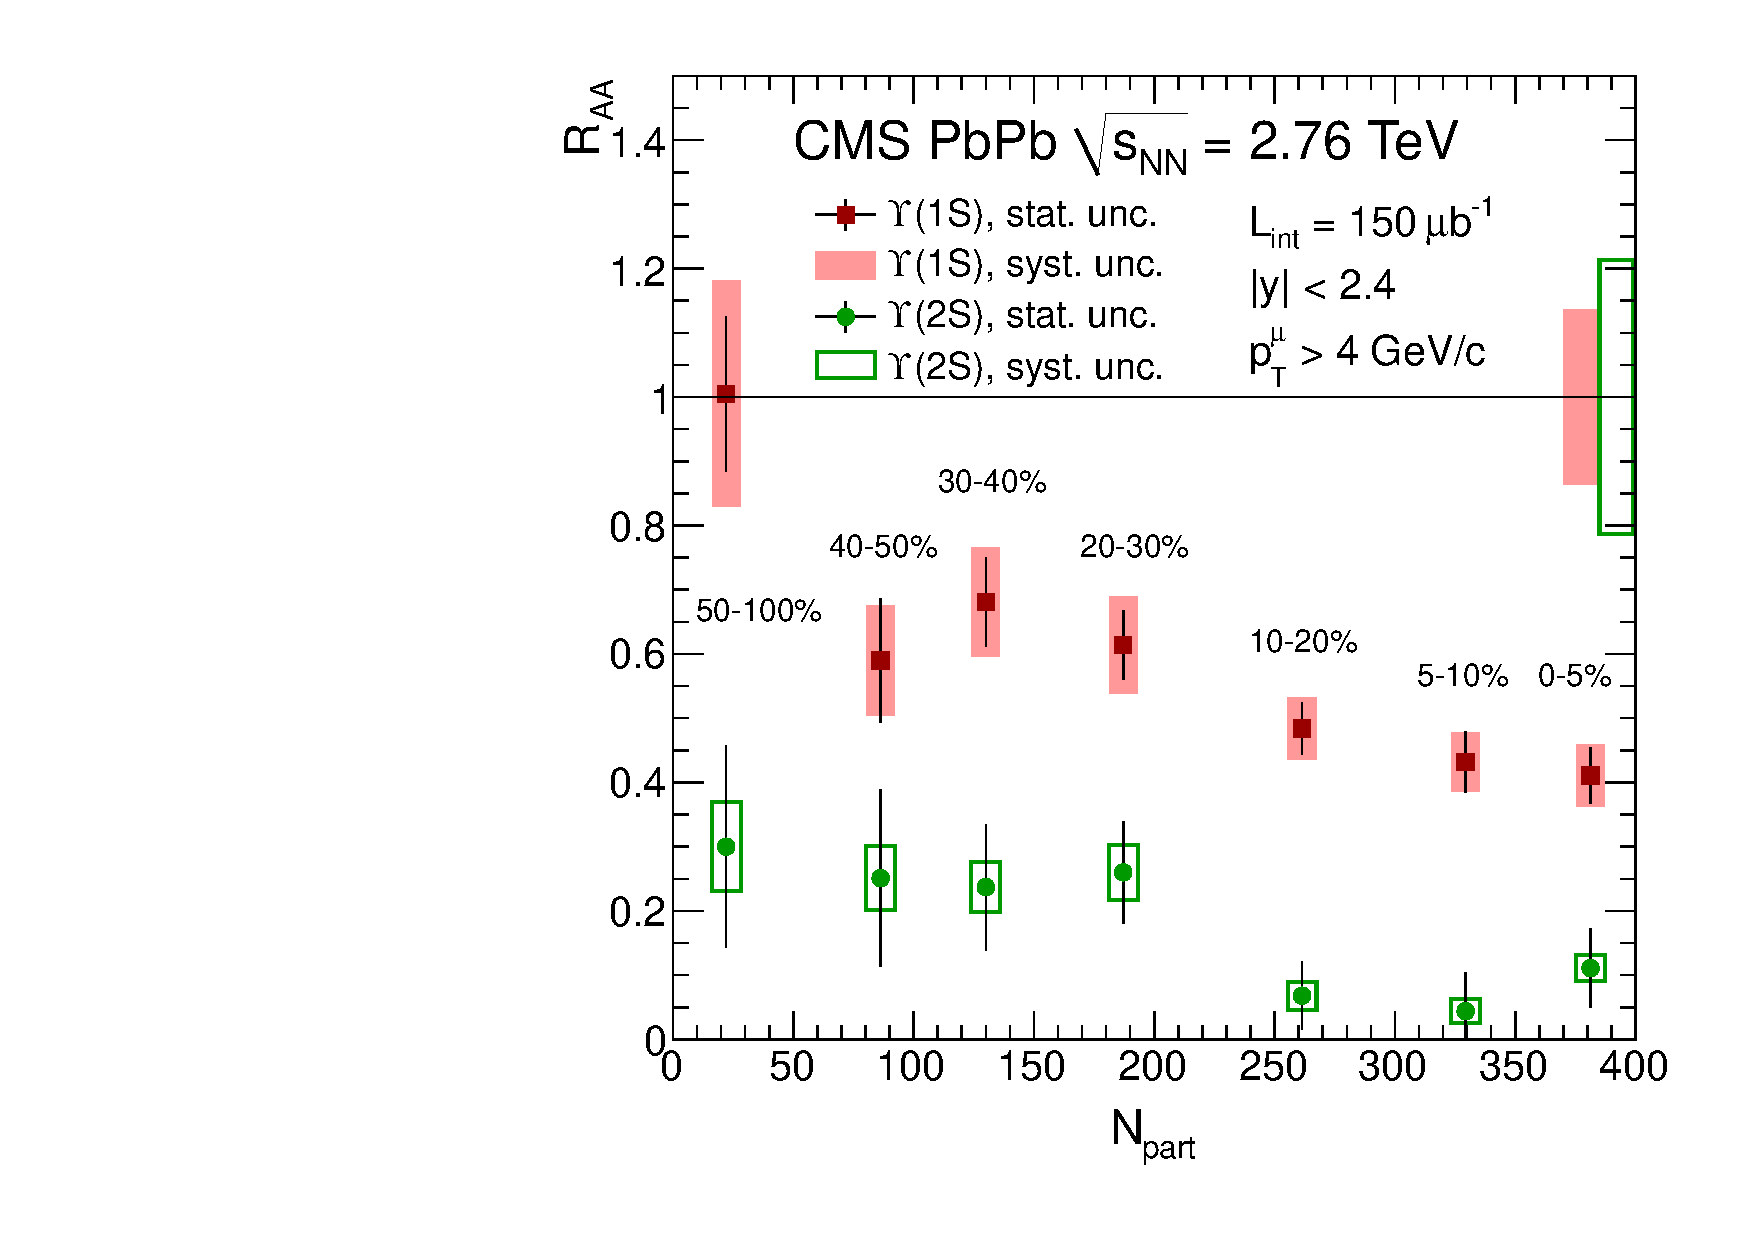
\includegraphics[width=0.45\textwidth]{qqbarfigures/RaaPt4}
  \caption{(left) Centrality dependence of the \PgUa\ and \PgUb\ double ratios
for 2.76\TeV\ collisions.  (right) Centrality dependence of \Raa\ 
for $\PgUa$ and $\PgUb$ for 2.76\TeV\ \PbPb\ collisions, relative to a \pp\ reference.
Error bars show statistical uncertainties, while the boxes around the markers
show systematic uncertainties. \npart-independent
common uncertainties are represented by the boxes at unity. Reproduced from~\cite{Chatrchyan:2012lxa}}.
\label{fig:GR:centrality}
\end{center}
\end{figure}

While \Raa\ shows a strongly falling trend with increasing collision centrality
for both \PgUa\ and \PgUb\ (with a much stronger suppression for \PgUb), the
double ratio does not exhibit a pronounced centrality dependence.

Overall, the CMS data qualitatively exhibit the hierarchy in the \PgUn\ suppression pattern
expected based on the states' binding energies. Although the most peripheral bin
is rather wide (50--100\%), it is interesting to observe the strong suppression of the
\PgUb\ relative to the \PgUa\ already for this bin. Future high statistics \PbPb\ data
should elucidate the onset of the \PgU\ suppression in the most peripheral collisions,
in combination with information on \PgU\ suppression in small systems obtained from
studies in \pPb\ reference data.

